\subsection{$k$-Regular Colourability Problem}

We show that the "$k$-regular colourability problem" is undecidable for $k\geq 2$.%
\footnote{
    Using this, we obtain in the next subsection 
    the undecidability for the separability problem on two natural classes of 
    "recognizable relations".
    On the other hand, the undecidability of "regular colourability problem" is more involved and will only come later, in todo:addref.
}
This is proven by a reduction from a suitable problem on reversible 
Turing machines with certain restrictions, which we call ``well-founded''.

\paragraph*{Regularity of Reachability for Turing Machines.}
Consider a Turing machine $\+T = \tup{Q,\Gamma,\delta,q_0,\Acc}$, where $Q$ is the set of states, $\Gamma$ is tape alphabet,
\[
    \delta\colon (Q \setminus \Acc) \times \Gamma_{\pad} \to \pset{Q \times \Gamma \times \set{\leftarrow, \downarrow, \rightarrow}}
\]
is the transition relation, $\Gamma_{\pad} = \Gamma \dcup \set{\pad}$, and $q_0$ and $\Acc$ are the initial and set of final states, respectively.
%
We represent a "configuration@@TM" $\tup{u, q, v}$ by the word $uqv \in \Gamma^* Q \Gamma^*$:
in light of this, we will henceforth denote by ``configuration'' any string from the set  \AP$\intro*\configs \defeq  \Gamma^* Q \Gamma^*$.\footnote{We will often write
$uqv$ as the concatenation $u\cdot q \cdot v$ to emphasize
the separation between all three words.}
The \AP""configuration graph"" of $\+T$ is the infinite graph $\intro*\confGraph$ having $\configs$ as set of vertices and an edge from $\gamma$ to $\gamma'$, denoted $\gamma \rightarrow \gamma'$ if there is a one-step transition from $\gamma$ to $\gamma'$ in $\+T$. Observe that the "configuration graph" $\confGraph$ of any Turing machine $\+T$ is an effective "rational graph" (see, e.g., \cite{KuskeLohrey2010AutomaticGraphs} TODO:update pointer to prelims).

\AP We say that a Turing machine $\+T$ is ""reversible"", if every node of $\confGraph$ has in-degree at most 1, in other words if the machine is co-deterministic.%
\footnote{
    Note that a modern proof of undecidability of the isomorphism problem for automatic structures 
    by Blumensath \cite[\S VIII. Theorem 4.3, p. 396 \& second claim, p. 398]{Blumensath2023MSO} 
    also relies on the use of "reversible" Turing machines.
}%
\footnote{
    For more details and pointers on "reversible" Turing machines,
    see \cite[Chapter 5]{Morita2017Reversible}.
}
We say that a Turing machine $\+T$ is ""well-founded"" if its "configuration graph" is such that:
\begin{enumerate}
    \item the "initial configuration" has in-degree zero, and
    \item there are no infinite backward paths $\gamma_0 \leftarrow \gamma_1 \leftarrow \cdots$ in $\confGraph$. 
\end{enumerate}

We say that a Turing machine is ""linear@@TM"" if it is "well-founded", deterministic and "reversible".
By construction, a Turing machine is "linear@@TM" "iff" (1) its "configuration graph" consists of a possibly infinite disjoint union of directed paths, which are all finite, or isomorphic to $\tup{\N, +1}$ and (2) the "initial configuration" has in-degree zero.
Such a configuration graph is depicted on
\Cref{fig:reduction-wf-RTM-to-colouring-config-graph-wf-RTM}.\footnote{Note
that it is decidable whether a "Turing machine" is "linear@@TM". In fact, condition (1) can be expressed in "first-order logic" over $\univStructSynchronous{\Sigma}$.}

\AP The ""reachable regularity problem"" is the problem of, given a "Turing machine" $\+T$, to decide whether its set of "reachable configurations" is a "regular language". To show that is it undecidable, we exhibit a reduction from the halting problem on deterministic "reversible" Turing machines.

\begin{proposition}[{\cite[Theorem 1]{Lecerf1963MachinesReversibles}}]
    \AP\label{prop:halting-problem-detrevTM}
    The \DPfont{halting problem} on deterministic "reversible" Turing machines is undecidable.
\end{proposition}

\begin{lemma}
    \AP\label{lem:reachable-regularity}
    The "reachable regularity problem" is undecidable, even if restricted
    to "linear Turing machines".
\end{lemma}

\begin{proof}[Proof sketch]
    We reduce the \DPfont{halting problem} on deterministic "reversible" Turing machines,
    in such a way that the "reachable configurations" whose
    state $q$ coincide with the state of the original machine are
    of the form $u \cdot q \cdot v \triangleright^n \triangleleft^n$ where $u \cdot q \cdot v$ is a configuration of the 
    original machine, $\triangleright$ and $\triangleleft$ are new symbols,
    and $n\in\N$. Transitions are defined in such a way that the new machine is
    "linear@@TM": this is implemented by having, for every transition $u\cdot q \cdot v \to u' \cdot q' \cdot v'$ of the original machine and every $n,m\in \N$, a multistep transition
    \[ 
        u \cdot q\cdot v \triangleright^{n} \triangleleft^{m} \to^* u' \cdot q' \cdot v' \triangleright^{n+1} \triangleleft^{m+1}.
    \]
    The construction is illustrated in \Cref{fig:reachable-regularity}.
	\begin{figure}[htb]
		\centering
        \begin{tikzpicture}
		    % ---
% First tape
% ---
\node (0) at (0,0) {0};
\node[right = 0cm of 0] (1) {0};
\node[right = 0cm of 1] (2) {1};
\node[right = 0cm of 2] (3) {0};
\node[right = 0cm of 3] (4) {1};
\node[right = 0cm of 4] (5) {$a\vphantom{b}$};
\node[right = 0cm of 5] (6) {$a\vphantom{b}$};
\node[right = 0cm of 6] (7) {$a\vphantom{b}$};
\node[right = 0cm of 7] (8) {$b$};
\node[right = 0cm of 8] (9) {$b$};
\node[right = 0cm of 9] (10) {$b$};

\draw[rounded corners=4pt] (0.south west) rectangle (10.north east);
\draw[->, thick] ($(5.north)+(0,.4)$) -- ($(5.north)+(0,.1)$);
\node[above=.05cm, circle, draw=cBlue, fill=cBlue, opacity=.5, text opacity=1, inner sep=1.5pt] at ($(5.north)+(0,.4)$) {$p$};

% ---
% Second tape
% ---
\node[below = 1.2cm of 0] (0') {0};
\node[right = 0cm of 0'] (1') {0};
\node[right = 0cm of 1'] (2') {1};
\node[right = 0cm of 2'] (3') {0};
\node[right = 0cm of 3'] (4') {1};
\node[right = 0cm of 4'] (5') {1};
\node[right = 0cm of 5'] (6') {$a\vphantom{b}$};
\node[right = 0cm of 6'] (7') {$a\vphantom{b}$};
\node[right = 0cm of 7'] (8') {$b$};
\node[right = 0cm of 8'] (9') {$b$};
\node[right = 0cm of 9'] (10') {$b$};

\draw[rounded corners=4pt] (0'.south west) rectangle (10'.north east);
\draw[->, thick] ($(6'.north)+(0,.4)$) -- ($(6'.north)+(0,.1)$);
\node[above=.05cm, circle, draw=cRed, fill=cRed, opacity=.5, text opacity=1, inner sep=1.5pt] at ($(6'.north)+(0,.4)$) {$\phantom{q}$};

% ---
% Third tape
% ---
\node[below = 1.2cm of 0'] (0'') {0};
\node[right = 0cm of 0''] (1'') {0};
\node[right = 0cm of 1''] (2'') {1};
\node[right = 0cm of 2''] (3'') {0};
\node[right = 0cm of 3''] (4'') {1};
\node[right = 0cm of 4''] (5'') {1};
\node[right = 0cm of 5''] (6'') {$a\vphantom{b}$};
\node[right = 0cm of 6''] (7'') {$a\vphantom{b}$};
\node[right = 0cm of 7''] (8'') {$a\vphantom{b}$};
\node[right = 0cm of 8''] (9'') {$a\vphantom{b}$};
\node[right = 0cm of 9''] (10'') {$b$};

\draw[rounded corners=4pt] (0''.south west) rectangle (10''.north east);
\draw[->, thick] ($(10''.north)+(0,.4)$) -- ($(10''.north)+(0,.1)$);
\node[above=.05cm, circle, draw=cRed, fill=cRed, opacity=.5, text opacity=1, inner sep=1.5pt] at ($(10''.north)+(0,.4)$) {$\phantom{q}$};

% ---
% Fourth tape
% ---
\node[below = 1.2cm of 0''] (0''') {0};
\node[right = 0cm of 0'''] (1''') {0};
\node[right = 0cm of 1'''] (2''') {1};
\node[right = 0cm of 2'''] (3''') {0};
\node[right = 0cm of 3'''] (4''') {1};
\node[right = 0cm of 4'''] (5''') {1};
\node[right = 0cm of 5'''] (6''') {$a\vphantom{b}$};
\node[right = 0cm of 6'''] (7''') {$a\vphantom{b}$};
\node[right = 0cm of 7'''] (8''') {$a\vphantom{b}$};
\node[right = 0cm of 8'''] (9''') {$a\vphantom{b}$};
\node[right = 0cm of 9'''] (10''') {$b$};
\node[right = 0cm of 10'''] (11''') {$b$};
\node[right = 0cm of 11'''] (12''') {$b$};
\node[right = 0cm of 12'''] (13''') {$b$};

\draw[rounded corners=4pt] (0'''.south west) rectangle (13'''.north east);
\draw[->, thick] ($(13'''.north)+(0,.4)$) -- ($(13'''.north)+(0,.1)$);
\node[above=.05cm, circle, draw=cRed, fill=cRed, opacity=.5, text opacity=1, inner sep=1.5pt] at ($(13'''.north)+(0,.4)$) {$\phantom{q}$};

% ---
% Fifth tape
% ---
\node[below = 1.2cm of 0'''] (0'''') {0};
\node[right = 0cm of 0''''] (1'''') {0};
\node[right = 0cm of 1''''] (2'''') {1};
\node[right = 0cm of 2''''] (3'''') {0};
\node[right = 0cm of 3''''] (4'''') {1};
\node[right = 0cm of 4''''] (5'''') {1};
\node[right = 0cm of 5''''] (6'''') {$a\vphantom{b}$};
\node[right = 0cm of 6''''] (7'''') {$a\vphantom{b}$};
\node[right = 0cm of 7''''] (8'''') {$a\vphantom{b}$};
\node[right = 0cm of 8''''] (9'''') {$a\vphantom{b}$};
\node[right = 0cm of 9''''] (10'''') {$b$};
\node[right = 0cm of 10''''] (11'''') {$b$};
\node[right = 0cm of 11''''] (12'''') {$b$};
\node[right = 0cm of 12''''] (13'''') {$b$};

\draw[rounded corners=4pt] (0''''.south west) rectangle (13''''.north east);
\draw[->, thick] ($(6''''.north)+(0,.4)$) -- ($(6''''.north)+(0,.1)$);
\node[above=.05cm, circle, draw=cBlue, fill=cBlue, opacity=.5, text opacity=1, inner sep=1.5pt] at ($(6''''.north)+(0,.4)$) {$q$};

% ---
% Transitions
% ---
\draw[->, dashed] ($(10.east)+(.3,-.2)$) to[bend left=50]
	node[midway, right=.15cm, align=left, text width=3.5cm, font=\footnotesize] {simulate $T$}
	($(10'.east)+(.3,.2)$);

\draw[->, dashed] ($(10'.east)+(.3,-.2)$) to[bend left=50]
	node[midway, right=.15cm, align=left, text width=3.5cm, font=\footnotesize]
		{overwrite the first two $b$'s with $a$'s}
	($(10''.east)+(.3,.2)$);

% \draw[-, dashed] ($(10''.east)+(.3,-.1)$) to ($(10''.east)+(1.5,-.1)$);
\draw[->, dashed] ($(10''.east)+(1.5,-.2)$) to[bend left=50]
	node[midway, right=.15cm, align=left, text width=3.5cm, font=\footnotesize]
		{append three $b$'s}
	($(13'''.east)+(.3,.2)$);


\draw[->, dashed] ($(13'''.east)+(.3,-.2)$) to[bend left=50]
	node[midway, right=.15cm, align=left, text width=3.5cm, font=\footnotesize]
		{go back to the new position, in the new state}
	($(13''''.east)+(.3,.2)$);
        \end{tikzpicture}
		\caption{
			\AP\label{fig:reachable-regularity}
			Encoding of a single transition of the form
			``when reading a blank in state $\color{cBlue} p$, write a
			$1$, go in state $\color{cBlue} q$ and move right''
			of the machine $T$ in the machine $T'$
			in the proof of \Cref{lem:reachable-regularity}.
			Red unlabelled states represent states of $T'$
			that are not originally present in $T$.
		}
	\end{figure}
	
    Moreover:
    \begin{itemize}
        \item if the original machine was halting, then the "reachable configurations"
            of the new one are finite and hence regular;
        \item otherwise, the set of "reachable configurations" is not regular,
            which follows from the non-regularity of any infinite subset of $\{\triangleright^n \triangleleft^n \mid n \in \N\}$.\qedhere
    \end{itemize}
\end{proof}

\begin{proof}[Some proof details]
    Letting $\+T$ denote the instance of the \DPfont{halting problem}, which runs on the empty word,
    we denote by $\+T'$ the instance of the "reachable regularity problem" to which it
    is reduced.

    $\+T'$ is defined as follows: every time there is a transition
    $u\cdot p \cdot v \to u' \cdot q \cdot v'$ in $\+T$,
	we simulate this transition in $T'$: to achieve this, `$\triangleright$' and `$\triangleleft$'s should be treated as blank symbols,
	and then we rewrite $\triangleright^n \triangleleft^m$ into $\triangleright^{n+1}\triangleleft^{m+1}$.
	When $\+T$ writes on a blank symbol that was actually an `$\triangleright$' in $\+T'$,
	we must also add an extra $\triangleright$ (to account for the one that was overwritten):
	this case is depicted in \Cref{fig:reachable-regularity}.
	Moreover, when $\+T$ deletes a symbol at the end of the tape,
	we must shift the $\triangleright^n \triangleright^m$ suffix. This can be done by replacing the blank
	with an `$\triangleright$', the last `$\triangleright$' with a `$\triangleleft$', and deleting the last `$\triangleleft$'.
	
    We now prove that $\+T'$ is "linear@@TM":
    \begin{enumerate}
        \item it is deterministic and "reversible":
        \begin{itemize}
            \item every "configuration" inside a path
            \[u \cdot q\cdot v \triangleright^{n} \triangleleft^{m} \to^* u' \cdot q' \cdot v' \triangleright^{n+1} \triangleleft^{m+1}\]
            has, by definition, exactly in- and out-degree one;
            \item every "configuration" of the form $u \cdot q \cdot v a^n b^m$ has as many 
            predecessors (resp. successors) in $\+T'$ as $u \cdot q \cdot v$ in $\+T$, namely one since $\+T$ was assumed to be deterministic and "reversible";
        \end{itemize}
        \item the "initial configuration" $\pad \cdot q_0 \cdot \pad$ has no predecessor;
        \item it has no infinite backward path since $\N$ is well-founded,
    \end{enumerate}
    Moreover, $\+T'$ has no cycle,\footnote{Indeed, we encoded a strictly increasing counter inside the configurations of $\+T'$.} and so if $\+T$ is halting on an empty input, then the set of "reachable configurations" of $\+T'$ is finite, and thus regular. If $\+T$ is not halting, the set of "reachable configurations" of $\+T'$ is infinite and its projection onto $\set{\triangleright,\triangleleft}$ is an infinite set of words of the form $a^{n} b^{m}$ where $n-2 \leq m \leq n+2$. Hence, since regular languages are closed under homomorphic images, the "reachable configurations" of $\+T'$ cannot be regular.
\end{proof}


\paragraph*{Undecidability of the $k$-Regular Colourability Problem.}
We can now show undecidability for the "$k$-regular colourability problem" by reduction from the "reachable regularity problem" restricted to "linear Turing machines".

\begin{marginfigure}
    \centering
    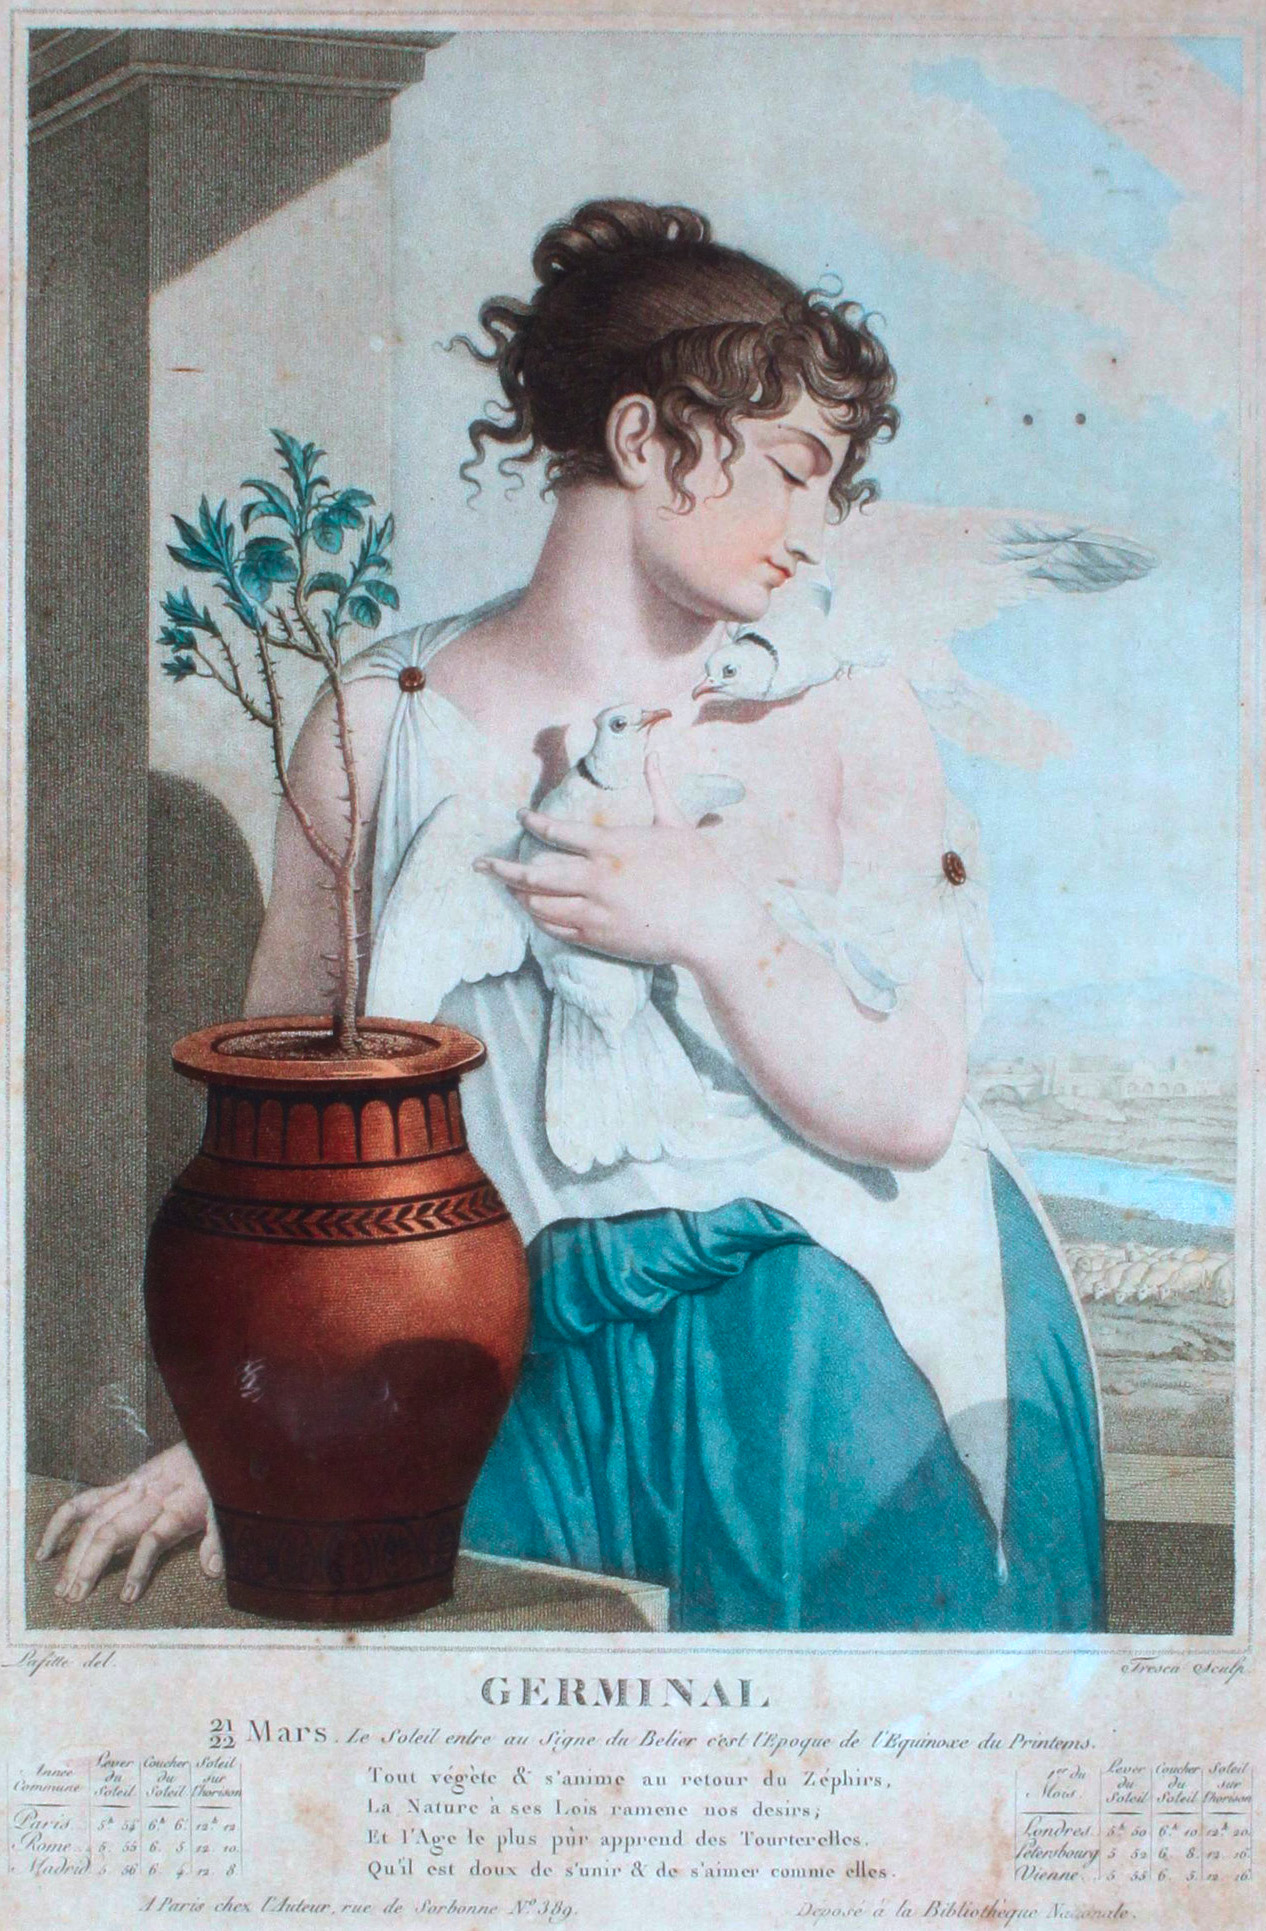
\includegraphics[width=\linewidth]{fig/germinal.jpg}
    \caption{\emph{Allégorie pour le mois de Germinal}, Louis Lafitte.}
\end{marginfigure}

A configuration of a "Turing machine"---or more generally the node of a "rational graph"---is said 
to be \AP""germinal"" if it has in-degree 0.
% \sidenote{A natural terminology would be ``initial'' but it clashes with the well-established notion of "initial configuration".}

\begin{theorem}
    \AP\label{thm:k-reg-col-undec}
    The "$k$-regular colourability problem" on "rational graphs" is undecidable, for every $k\geq 2$. More precisely, the problem is "RE"-complete. This holds also for "connected" "rational graphs".
\end{theorem}

\begin{proof}%
	\proofcase{Lower bound.}
    By reduction from the "reachable regularity problem" for "linear Turing machines"
    (\Cref{lem:reachable-regularity}). We first show it for $k=2$.

    \AP Given a "linear Turing machine" $T$,
    observe that the set $\intro*\Germ$ of all "germinal configurations" of $\confGraph$.
    \begin{claim}
        $\Germ$ is effectively a "regular language". 
    \end{claim}
    
    Observe moreover that, by definition of "linear Turing machines",
    the "initial configuration" $\pad\cdot q_0 \cdot \pad$ is "germinal".
    Let $\bSymb$ and $\rSymb$ be fresh symbols. 
    Consider the "rational graph" $\AutGraph{V}{\+E}$ for $V \defeq \configs\cdot (\bSymb + \rSymb)$,
    having an edge from $\gamma \cdot c$ to $\gamma' \cdot c$ if either 
    \begin{enumerate}
        \item $\tup{c,c'} = \tup{\bSymb,\rSymb}$ and $\gamma=\gamma'$;
        \item $\tup{c,c'} = \tup{\rSymb,\bSymb}$ and there is an edge from $\gamma$ to $\gamma'$ in $\confGraph$; or
        \item $\tup{c,c'} = \tup{\bSymb,\bSymb}$, $\gamma$ is the "initial configuration",
        and $\gamma' \neq \gamma$ is "germinal".
    \end{enumerate}

    \begin{marginfigure}%
        \centering
        \begin{tikzpicture}
            % Reachable configuration
\fill[rounded corners, draw=cGreen, fill=cGreen, opacity=.3]
	(-.3,-.3) rectangle (2.75, .3);
% Initial configuration
\fill[rounded corners, draw=cYellow, fill=cYellow, opacity=.3]
	(-.3,.3) rectangle (.3, -1.95);

% First line
\node[vertex] (a0) at (0,0) {};
\foreach \i in {0,...,2} {
	\pgfmathtruncatemacro{\next}{\i + 1}
	\node[vertex, right = of a\i] (a\next) {};
	\draw[edge] (a\i) to (a\next);
}

% Second line
\node[vertex, below = of a0] (b0) {};
\foreach \i in {0,...,3} {
	\pgfmathtruncatemacro{\next}{\i + 1}
	\node[vertex, right = of b\i] (b\next) {};
	\draw[edge] (b\i) to (b\next);
}
\node[draw=none, fill=none, right = 0cm of b4] (binf) {$\cdots$};

% Third line
\node[vertex, below = of b0] (c0) {};
\foreach \i in {0,1} {
	\pgfmathtruncatemacro{\next}{\i + 1}
	\node[vertex, right = of c\i] (c\next) {};
	\draw[edge] (c\i) to (c\next);
}

% Labels
\node[draw=none, fill=none, font=\small] [below = 1em of c0] {$\GermC{cYellow}$};
\node[draw=none, fill=none, font=\small, align=center] [above = 1em of $(a1)!0.5!(a2)$]
	{$\ReachC{\+T}{cGreen}$};
        \end{tikzpicture}
        \caption{
            \AP\label{fig:reduction-wf-RTM-to-colouring-config-graph-wf-RTM}
            Configuration graph of a "linear Turing machine".
        }
    \end{marginfigure}%
    \begin{marginfigure}%
        \centering
        \begin{tikzpicture}
            
% Reachable configuration
\fill[rounded corners, draw=cGreen, fill=cGreen, opacity=.3]
	(-.3,-.9) rectangle (2.75, .3);
% Initial configuration
\fill[rounded corners, draw=cYellow, fill=cYellow, opacity=.3]
	(-.3,.3) rectangle (.3, -3.8);

% First line
\node[vertex, cBlue, fill=cBlue, fill opacity=.4] (a0) at (0,0) {};
\node[vertex, cRed, fill=cRed, fill opacity=.4] (a'0) [below = .3cm of a0] {};
\draw[edge, densely dotted] (a0) to (a'0);
\foreach \i in {0,...,2} {
	\pgfmathtruncatemacro{\next}{\i + 1}
	\node[vertex, cBlue, fill=cBlue, fill opacity=.4, right = of a\i] (a\next) {};
	\node[vertex, cRed, fill=cRed, fill opacity=.4, right = of a'\i] (a'\next) {};
	\draw[edge] (a'\i) to (a\next);
	\draw[edge, densely dotted] (a\next) to (a'\next);
}

% Second line
\node[vertex, cBlue, fill=cBlue, fill opacity=.4, below = of a'0] (b0) {};
\node[vertex, cRed, fill=cRed, fill opacity=.4, below =.3cm of b0] (b'0) {};
\draw[edge, densely dotted] (b0) to (b'0);
\foreach \i in {0,...,3} {
	\pgfmathtruncatemacro{\next}{\i + 1}
	\node[vertex, cBlue, fill=cBlue, fill opacity=.4, right = of b\i] (b\next) {};
	\node[vertex, cRed, fill=cRed, fill opacity=.4, right = of b'\i] (b'\next) {};
	\draw[edge] (b'\i) to (b\next);
	\draw[edge, densely dotted] (b\next) to (b'\next);
}
\node[draw=none, fill=none, right = .6em of $(b4)!0.5!(b'4)$] (binf) {$\cdots$};

% Third line
\node[vertex, cBlue, fill=cBlue, fill opacity=.4, below = of b'0] (c0) {};
\node[vertex, cRed, fill=cRed, fill opacity=.4, below = .3cm of c0] (c'0) {};
\draw[edge, densely dotted] (c0) to (c'0);
\foreach \i in {0,1} {
	\pgfmathtruncatemacro{\next}{\i + 1}
	\node[vertex, cBlue, fill=cBlue, fill opacity=.4, right = of c\i] (c\next) {};
	\node[vertex, cRed, fill=cRed, fill opacity=.4, right = of c'\i] (c'\next) {};
	\draw[edge] (c'\i) to (c\next);
	\draw[edge, densely dotted] (c\next) to (c'\next);
}

% Edges between Init nodes
\draw[edge, densely dashed] (a0) to[bend right] (b0);
\draw[edge, densely dashed] (a0) to[bend right] (c0);

% Labels
\node[draw=none, fill=none, cYellow, font=\footnotesize, align=left]
	[below right = 1em and -1em of $(c'0)$]
	{nodes originating from	$\InitC{cYellow}$};
\node[draw=none, fill=none, cGreen, font=\footnotesize, align=left]
	[above right = 1em and -1em of $(a0)$]
	{nodes originating from $\ReachC{cGreen}$};
        \end{tikzpicture}
        \caption{
            \AP\label{fig:reduction-wf-RTM-to-colouring}
            The "rational graph" to which the "configuration graph"
            of \Cref{fig:reduction-wf-RTM-to-colouring-config-graph-wf-RTM} is reduced.
        }
    \end{marginfigure}%

    Symbols $\bSymb$ and $\rSymb$ are utilized to represent two versions of each configuration.
    This graph is depicted in \Cref{fig:reduction-wf-RTM-to-colouring}.
    Note that $\AutGraph{V}{\+E}$ is "connected" and "2-colourable": in fact, it is a "directed tree" whose root is $\pad\cdot q_0\cdot \pad\cdot \bSymb$. 
    
    We claim that $\AutGraph{V}{\+E}$ is "$2$-regular colourable" if, and only if, the set of "reachable configurations" of $T$ is a "regular language". 
    In fact, up to permuting the two-colours, $\AutGraph{V}{\+E}$
    admits a unique 2-colouring $\tup{C_1,C_2}$, defined by:
    \[
        C_1 \defeq \Reach\cdot\bSymb \cup (\configs \setminus \Reach)\cdot\rSymb
    \]
    and $C_2$ is the complement of $C_1$.
    If $\Reach$ is regular, then so is $C_1$. Dually, if $C_1$ is regular, then
    $\Reach$ is exactly the set of configurations $\gamma$ such that
    $\gamma\cdot \bSymb \in C_1$ and hence is regular.
    It follows that $\AutGraph{V}{\+E}$ is "$2$-regular colourable" if and only if
    the "reachable configurations" of $\+T$ are regular, which concludes the proof for $k=2$.

    To prove the statement for any $k>2$, we define $\AutGraph{V}{\+E_k}$ as the result of adding a $(k-2)$-clique to $\AutGraph{V}{\+E}$ and adding an edge from every vertex of the clique to every vertex incident to an edge of $\+E$. This forces the clique to use $k-2$ colours that cannot be used in the remaining part of the graph and the proof is then analogous.

	\proofcase{Upper-bound.} We show that the problem is "RE". Let us define a \AP""$k$-coloured automaton"" like a regular (complete) DFA, except that instead of having
	a set of final states, it has a partition $\langle C_1,\hdots,C_k \rangle$ of its states.
	Such an automaton recognizes a "regular colouring" $\Sigma^* \to \lBrack 1, k\rBrack$.
	Given a "rational graph" $\+G = \AutGraph{V}{\+E}$---whose edge relations is given by
    a "synchronous automaton" $\relPres{\+E}{\+G}$---and a $k$-coloured automaton $\+B$,
	we can build, by a product construction, an automaton $\+A'$ which accepts
	all $u \otimes v \in \convolRel{R}$ such that the colour of $u$ is distinct from
    the colour of $v$.
	Then, $\+A'$ is equivalent to $\relPres{\+E}{\+G}$ if, and only if,
    $\+B$ describes a proper "$k$-colouring" of $\AutGraph{V}{\+E}$.
    The "RE" upper-bound of the "$k$-regular colourability problem" follows: 
    it suffices to enumerate all "$k$-coloured automata" and check for equivalence.
\end{proof}

Note that this reduction provides an easy way of building
graphs in the shape of \Cref{fig:reduction-wf-RTM-to-colouring} that are "2-colourable" (in fact, they are trees) but not "2-regular colourable". In fact, we can provide a slightly more
direct construction.

\begin{example}
    \AP\label{ex:tree-not-2-reg-colourable}
    On the alphabet $\Sigma = \{a,b\}$, the tree $\+T$ depicted in \Cref{fig:tree-not-2reg-colour} whose set of vertices is $V = a^*b^*$ and whose set 
    of edges is $\+E = \+E_{\mathrm{incr}} \cup \+E_{\mathrm{init}}$, with 
    \begin{align*}
        \+E_{\mathrm{incr}} & = \{(a^pb^q,\, a^{p+1}b^{q+1}) \mid p,q \in \N\} \\
        \+E_{\mathrm{init}} & = \{(\varepsilon,\, a^p) \mid p \in \N\} \cup \{(\varepsilon,\, b^q) \mid q \in \N\}, 
    \end{align*}    
    is "rational@@rational graph" but not "2-regular colourable".
    Indeed, its only "2-colouring"
    consists in partitioning the vertices of $\+T$ into
    \begin{align*}
        C =\;& \{a^n b^n \mid n \in 2\N\} \\
            & \cup \{a^p b^q \mid p > q \text{ and $q$ is odd}\} \\
            & \cup \{a^p b^q \mid p < q \text{ and $p$ is odd}\}
    \end{align*}
    and its complement $V \setminus C$.
    Let $P = \{a^p b^q \mid p, q \in 2\N\} = (aa)^*(bb)^*$:
    $P$ is regular, yet $C \cap P = \{a^n b^n \mid n \in 2\N\}$ is not.
    Hence, $C$ is not regular, and thus $\+T$ is not "2-regular colourable".
\end{example}

\begin{figure}
    \centering
    \begin{tikzpicture}
        % Coloring
\fill[rounded corners, fill=cBlue, opacity=.5]
	(-.4,-0.25) rectangle (.4,0.23)
	(2.1,-0.25) rectangle (2.9,0.23)
	(0.85,-0.52) rectangle (1.65, -2.5)
	(3.35,-0.52) rectangle (4.15, -2.5);

\fill[rounded corners, fill=cRed, opacity=.5, xshift=1.25cm]
	(-.4,-0.25) rectangle (.4,0.23)
	(2.1,-0.25) rectangle (2.9,0.23);
\fill[rounded corners, fill=cRed, opacity=.5, xshift=-1.25cm]
	(0.85,-0.52) rectangle (1.65, -2.5)
	(3.35,-0.52) rectangle (4.15, -2.5);

% Tree
\node (eps) at (0,0) {$\varepsilon$};
\node (ab) at (1.25,0) {$ab$};
\node (aabb) at (2.5,0) {$a^2b^2$};
\node (aaabbb) at (3.75,0) {$a^3b^3$};

\node (a) at (0,-.75) {$a$};
\node (aab) at (1.25,-.75) {$aab$};
\node (aaabb) at (2.5,-.75) {$a^3b^2$};
\node (aaaabbb) at (3.75,-.75) {$a^4b^3$};

\node (b) at (0,-1.5) {$b$};
\node (abb) at (1.25,-1.5) {$abb$};
\node (aabbb) at (2.5,-1.5) {$a^2b^3$};
\node (aaabbbb) at (3.75,-1.5) {$a^3b^4$};

\node (aa) at (0,-2.25) {$aa$};
\node (aaab) at (1.25,-2.25) {$a^3b$};
\node (aaaabb) at (2.5,-2.25) {$a^4b^2$};
\node (aaaaabbb) at (3.75,-2.25) {$a^5b^3$};

\draw[->] (eps) to (ab);
\draw[->] (ab) to (aabb);
\draw[->] (aabb) to (aaabbb);
\draw[->, dashed] (aaabbb) to ($(aaabbb)+(1,0)$);

\draw[->] (a) to (aab);
\draw[->] (aab) to (aaabb);
\draw[->] (aaabb) to (aaaabbb);
\draw[->, dashed] (aaaabbb) to ($(aaaabbb)+(1,0)$);

\draw[->] (b) to (abb);
\draw[->] (abb) to (aabbb);
\draw[->] (aabbb) to (aaabbbb);
\draw[->, dashed] (aaabbbb) to ($(aaabbbb)+(1,0)$);

\draw[->] (aa) to (aaab);
\draw[->] (aaab) to (aaaabb);
\draw[->] (aaaabb) to (aaaaabbb);
\draw[->, dashed] (aaaaabbb) to ($(aaaaabbb)+(1,0)$);

\draw[->] (eps) edge[bend right=40] (a)
	edge[bend right=40] (b)
	edge[bend right=40] (aa)
	edge[dashed, bend right=40] ($(aa)+(0,-.75)$);

\node[below = .25cm of aaab, color=cBlue] {$C$}; 
\node[below = .25cm of aaaabb, color=cRed] {$V \setminus C$}; 
    \end{tikzpicture}
    \caption{
        \label{fig:tree-not-2reg-colour}
        The "rational tree@rational graph" $\+T$ of \Cref{ex:tree-not-2-reg-colourable},
        and its unique "2-colouring" $(C, V\setminus C)$, which is not "regular@@colouring".
    }
\end{figure}